%package list
\documentclass{article}
\usepackage[top=3cm, bottom=3cm, outer=3cm, inner=3cm]{geometry}
\usepackage{graphicx}
\usepackage{url}
%\usepackage{cite}
\usepackage{hyperref}
\usepackage{array}
\usepackage{multicol}
\newcolumntype{x}[1]{>{\centering\arraybackslash\hspace{0pt}}p{#1}}
%\usepackage{natbib}
\usepackage{pdfpages}
\usepackage{multirow}
\usepackage{float}
\usepackage[shortlabels]{enumitem}
\usepackage{booktabs}
\usepackage{amssymb}
\usepackage[normalem]{ulem}
\useunder{\uline}{\ul}{}

\usepackage{listings}
\usepackage{xcolor}
\usepackage{algorithm,algorithmic}

\definecolor{codegreen}{rgb}{0,0.6,0}
\definecolor{codegray}{rgb}{0.5,0.5,0.5}
\definecolor{codepurple}{rgb}{0.58,0,0.82}
\definecolor{backcolour}{rgb}{0.95,0.95,0.92}

\lstdefinestyle{style_code}{
    backgroundcolor=\color{backcolour},   
    commentstyle=\color{codegreen},
    keywordstyle=\color{magenta},
    numberstyle=\tiny\color{codegray},
    stringstyle=\color{codepurple},
    basicstyle=\ttfamily\footnotesize,
    breakatwhitespace=false,         
    breaklines=true,                 
    captionpos=b,                    
    keepspaces=true,                 
    numbers=left,                    
    numbersep=5pt,                  
    showspaces=false,                
    showstringspaces=false,
    showtabs=false,                  
    tabsize=2
}

\lstset{style=style_code}

%%%%%%%%%%%%%%%%%%%%%%%%%%%%%%%%%%%%%%%%%%%%%%%%%%%%%%%%%%%%%%%%%%%%%%%%%%%%
%%%%%%%%%%%%%%%%%%%%%%%%%%%%%%%%%%%%%%%%%%%%%%%%%%%%%%%%%%%%%%%%%%%%%%%%%%%%
\newcommand{\csemail}{mquispecr@unsa.edu.pe}
\newcommand{\csdocente}{Marcela Quispe Cruz}
\newcommand{\cscurso}{Teoría de la Computación}
\newcommand{\csuniversidad}{Universidad Nacional de San Agustín}
\newcommand{\csescuela}{Maestría en Ciencia de la Computación}
\newcommand{\cspracnr}{03}
\newcommand{\cstema}{Lenguajes de Libre Contexto}
%%%%%%%%%%%%%%%%%%%%%%%%%%%%%%%%%%%%%%%%%%%%%%%%%%%%%%%%%%%%%%%%%%%%%%%%%%%%
%%%%%%%%%%%%%%%%%%%%%%%%%%%%%%%%%%%%%%%%%%%%%%%%%%%%%%%%%%%%%%%%%%%%%%%%%%%%


\usepackage[english,spanish]{babel}
\usepackage[utf8]{inputenc}
\AtBeginDocument{\selectlanguage{spanish}}
\renewcommand{\figurename}{Figura}
\renewcommand{\refname}{Referencias}
\renewcommand{\tablename}{Tabla} %esto no funciona cuando se usa babel
\AtBeginDocument{%
	\renewcommand\tablename{Tabla}
}

\usepackage{fancyhdr}
\pagestyle{fancy}
\fancyhf{}
\setlength{\headheight}{30pt}
\renewcommand{\headrulewidth}{1pt}
\renewcommand{\footrulewidth}{1pt}
\fancyhead[L]{\raisebox{-0.2\height}{
\includegraphics[width=3cm]{img/logo_unsa}}}
\fancyhead[C]{}
\fancyhead[R]{\fontsize{7}{7}\selectfont	\csuniversidad \\ \csescuela \\ \textbf{\cscurso} }
\fancyfoot[L]{Dra. Marcela Quispe Cruz}
\fancyfoot[C]{\cscurso}
\fancyfoot[R]{Página \thepage}




\begin{document}
	
	\vspace*{10px}
	
	\begin{center}	
		\fontsize{17}{17} \textbf{ Práctica \cspracnr}
	\end{center}
	%\centerline{\textbf{\underline{\Large Título: Informe de revisión del estado del arte}}}
	%\vspace*{0.5cm}
	

	\begin{table}[h]
		\begin{tabular}{|x{4.7cm}|x{4.8cm}|x{4.8cm}|}
			\hline 
			\textbf{DOCENTE} & \textbf{CARRERA}  & \textbf{CURSO}   \\
			\hline 
			\csdocente & \csescuela & \cscurso    \\
			\hline 
		\end{tabular}
	\end{table}	
	
	
	\begin{table}[h]
		\begin{tabular}{|x{4.7cm}|x{4.8cm}|x{4.8cm}|}
			\hline 
			\textbf{PRÁCTICA} & \textbf{TEMA}  & \textbf{DURACIÓN}   \\
			\hline 
			\cspracnr & \cstema & 3 horas   \\
			\hline 
		\end{tabular}
	\end{table}
	
	
	\section{Datos de los estudiantes}
	\begin{itemize}
		\item Grupo: 9
		\item Integrantes: 
		\begin{itemize}
			\item Abarca Murillo, Jhonatan Piero
			\item Apari Pinto, Christian Timoteo
			\item Suca Velando, Christian Anthony
			\item Vargas Zuni, Arturo
		\end{itemize}
		%\item Repositorio: \url{https://github.com/jabarcamu/}
	\end{itemize}
	

	
	\section{Ejercicios}\label{sec:ejercicios}
	
	\subsection{Pregunta 1}
	Considere las siguiente gramáticas:
	
	\begin{multicols}{2}
        \begin{enumerate}
            \item $S \to AbS|a, A \to a$
            \item $S \to Sa|AB, A \to aA|a, B \to b$
            \item $S \to aS|b$
            \item $S \to aS|aA, A \to bS|bA|\epsilon$
            \item $S \to aSa|b$
            \item $S \to aA|aS, A \to ab$
            \item $S \to ASB|AB, A \to aA|\epsilon, B \to b$
            \item $S \to Ab, A \to AA|a$
            \item $S \to AS|b, A \to AA|a$
        \end{enumerate}
    \end{multicols}
    
    Indique cual gramática corresponde a cada lenguaje abajo. Puede haber más de una o ninguna gramática para cada lenguaje.
    
    \begin{enumerate} [(a)]
        \item $ L_1 : \{a^ib | i \geq 1\}$ \dotfill  %\makebox[0pt][l]{$\square$}\raisebox{.15ex}{\hspace{0.1em}$\checkmark$} 1 
         \hspace{0.8em}{$\square$}\raisebox{.15ex}{\hspace{0.1em}} 1  \hspace{0.8em}\makebox[0pt][l]{$\square$}\raisebox{.15ex}{\hspace{0.1em}$\checkmark$} 2  \hspace{0.8em}\makebox[0pt][l]{$\square$}\raisebox{.15ex}{\hspace{0.1em}$\checkmark$} 3  \hspace{0.8em}\makebox[0pt][l]{$\square$}\raisebox{.15ex}{\hspace{0.1em}$\checkmark$} 4  \hspace{0.8em}{$\square$}\raisebox{.15ex}{\hspace{0.1em}} 5  \hspace{0.8em}{$\square$}\raisebox{.15ex}{\hspace{0.1em}} 6  \hspace{0.8em}\makebox[0pt][l]{$\square$}\raisebox{.15ex}{\hspace{0.1em}$\checkmark$} 7  \hspace{0.8em}\makebox[0pt][l]{$\square$}\raisebox{.15ex}{\hspace{0.1em}$\checkmark$} 8 
         \hspace{0.8em}\makebox[0pt][l]{$\square$}\raisebox{.15ex}{\hspace{0.1em}$\checkmark$} 9 
        
        \item $ L_2 : \{(ab)^ia | i \geq 0\}$ \dotfill  %\makebox[0pt][l]{$\square$}\raisebox{.15ex}{\hspace{0.1em}$\checkmark$} 1 
        \hspace{0.8em}\makebox[0pt][l]{$\square$}\raisebox{.15ex}{\hspace{0.1em}$\checkmark$} 1  \hspace{0.8em}{$\square$}\raisebox{.15ex}{\hspace{0.1em}} 2  \hspace{0.8em}{$\square$}\raisebox{.15ex}{\hspace{0.1em}} 3  \hspace{0.8em}\makebox[0pt][l]{$\square$}\raisebox{.15ex}{\hspace{0.1em}$\checkmark$} 4  \hspace{0.8em}{$\square$}\raisebox{.15ex}{\hspace{0.1em}} 5  \hspace{0.8em}{$\square$}\raisebox{.15ex}{\hspace{0.1em}} 6  \hspace{0.8em}{$\square$}\raisebox{.15ex}{\hspace{0.1em}} 7  \hspace{0.8em}{$\square$}\raisebox{.15ex}{\hspace{0.1em}} 8 
         \hspace{0.8em}{$\square$}\raisebox{.15ex}{\hspace{0.1em}} 9
        
        \item  $ L_3 : \{a^ib | i \geq 2\}$ \dotfill  %\makebox[0pt][l]{$\square$}\raisebox{.15ex}{\hspace{0.1em}$\checkmark$} 1 
        \hspace{0.8em}{$\square$}\raisebox{.15ex}{\hspace{0.1em}} 1  \hspace{0.8em}\makebox[0pt][l]{$\square$}\raisebox{.15ex}{\hspace{0.1em}$\checkmark$} 2  \hspace{0.8em}\makebox[0pt][l]{$\square$}\raisebox{.15ex}{\hspace{0.1em}$\checkmark$} 3  \hspace{0.8em}\makebox[0pt][l]{$\square$}\raisebox{.15ex}{\hspace{0.1em}$\checkmark$} 4  \hspace{0.8em}{$\square$}\raisebox{.15ex}{\hspace{0.1em}} 5  \hspace{0.8em}\makebox[0pt][l]{$\square$}\raisebox{.15ex}{\hspace{0.1em}$\checkmark$} 6  \hspace{0.8em}\makebox[0pt][l]{$\square$}\raisebox{.15ex}{\hspace{0.1em}$\checkmark$} 7  \hspace{0.8em}\makebox[0pt][l]{$\square$}\raisebox{.15ex}{\hspace{0.1em}$\checkmark$} 8 
         \hspace{0.8em}\makebox[0pt][l]{$\square$}\raisebox{.15ex}{\hspace{0.1em}$\checkmark$} 9
        
        \item $ L_4 : \{a^iba^j| i \geq 1, j \geq 0\}$ \dotfill  %\makebox[0pt][l]{$\square$}\raisebox{.15ex}{\hspace{0.1em}$\checkmark$} 1 
        \hspace{0.8em}{$\square$}\raisebox{.15ex}{\hspace{0.1em}} 1  \hspace{0.8em}\makebox[0pt][l]{$\square$}\raisebox{.15ex}{\hspace{0.1em}$\checkmark$} 2  \hspace{0.8em}{$\square$}\raisebox{.15ex}{\hspace{0.1em}} 3  \hspace{0.8em}\makebox[0pt][l]{$\square$}\raisebox{.15ex}{\hspace{0.1em}$\checkmark$} 4  \hspace{0.8em}{$\square$}\raisebox{.15ex}{\hspace{0.1em}} 5  \hspace{0.8em}{$\square$}\raisebox{.15ex}{\hspace{0.1em}} 6  \hspace{0.8em}{$\square$}\raisebox{.15ex}{\hspace{0.1em}} 7  \hspace{0.8em}{$\square$}\raisebox{.15ex}{\hspace{0.1em}} 8 
         \hspace{0.8em}{$\square$}\raisebox{.15ex}{\hspace{0.1em}} 9
        
        \item $ L_5 : \{a^ib | i \geq 0\}$ \dotfill  %\makebox[0pt][l]{$\square$}\raisebox{.15ex}{\hspace{0.1em}$\checkmark$} 1 
        \hspace{0.8em}{$\square$}\raisebox{.15ex}{\hspace{0.1em}} 1  \hspace{0.8em}{$\square$}\raisebox{.15ex}{\hspace{0.1em}} 2  \hspace{0.8em}\makebox[0pt][l]{$\square$}\raisebox{.15ex}{\hspace{0.1em}$\checkmark$} 3  \hspace{0.8em}{$\square$}\raisebox{.15ex}{\hspace{0.1em}} 4  \hspace{0.8em}{$\square$}\raisebox{.15ex}{\hspace{0.1em}} 5  \hspace{0.8em}{$\square$}\raisebox{.15ex}{\hspace{0.1em}} 6  \hspace{0.8em}\makebox[0pt][l]{$\square$}\raisebox{.15ex}{\hspace{0.1em}$\checkmark$} 7  \hspace{0.8em}{$\square$}\raisebox{.15ex}{\hspace{0.1em}} 8 
         \hspace{0.8em}\makebox[0pt][l]{$\square$}\raisebox{.15ex}{\hspace{0.1em}$\checkmark$} 9
         
        \item  $ L_6 : \{a^ib^j| i \geq 0, j > 0\}$ \dotfill 
        %\makebox[0pt][l]{$\square$}\raisebox{.15ex}{\hspace{0.1em}$\checkmark$} 1 
        \hspace{0.8em}{$\square$}\raisebox{.15ex}{\hspace{0.1em}} 1  \hspace{0.8em}{$\square$}\raisebox{.15ex}{\hspace{0.1em}} 2  \hspace{0.8em}{$\square$}\raisebox{.15ex}{\hspace{0.1em}} 3  \hspace{0.8em}{$\square$}\raisebox{.15ex}{\hspace{0.1em}} 4  \hspace{0.8em}{$\square$}\raisebox{.15ex}{\hspace{0.1em}} 5  \hspace{0.8em}{$\square$}\raisebox{.15ex}{\hspace{0.1em}} 6  \hspace{0.8em}\makebox[0pt][l]{$\square$}\raisebox{.15ex}{\hspace{0.1em}$\checkmark$} 7  \hspace{0.8em}{$\square$}\raisebox{.15ex}{\hspace{0.1em}} 8 
         \hspace{0.8em}{$\square$}\raisebox{.15ex}{\hspace{0.1em}} 9
        \item $ L_7 : \{(ab)^i| i \geq 0\}$ \dotfill \hspace{0.8em}{$\square$}\raisebox{.15ex}{\hspace{0.1em}} 1  \hspace{0.8em}{$\square$}\raisebox{.15ex}{\hspace{0.1em}} 2  \hspace{0.8em}{$\square$}\raisebox{.15ex}{\hspace{0.1em}} 3  \hspace{0.8em}{$\square$}\raisebox{.15ex}{\hspace{0.1em}} 4  \hspace{0.8em}{$\square$}\raisebox{.15ex}{\hspace{0.1em}} 5  \hspace{0.8em}{$\square$}\raisebox{.15ex}{\hspace{0.1em}} 6  \hspace{0.8em}{$\square$}\raisebox{.15ex}{\hspace{0.1em}} 7  \hspace{0.8em}{$\square$}\raisebox{.15ex}{\hspace{0.1em}} 8 
         \hspace{0.8em}{$\square$}\raisebox{.15ex}{\hspace{0.1em}} 9

    \end{enumerate}
    
    \textbf{Resolución}\\
    
    \textbf{Parte 1} Representando lenguajes \cite{sipser13}
    
    \begin{enumerate} [(a)]
        \item   $ L_1 : \{a^ib | i \geq 1\}$ \\
                $ L_1 : \{ab, aab, aaab, aaaab\}$   
        \item   $ L_2 : \{(ab)^ia | i \geq 0\}$ \\
                $ L_2 : \{a, aba, ababa, abababa\}$   
        \item   $ L_3 : \{a^ib | i \geq 2\}$ \\
                $ L_3 : \{aab, aaab, aaaab, aaaaab\}$
        \item   $ L_4 : \{a^iba^j| i \geq 1, j \geq 0\}$ \\
                $ L_4 : \{ab, aba, aaba, aabaa\}$
        \item   $ L_5 : \{a^ib | i \geq 0\}$ \\
                $ L_5 : \{b, ab, aab, aaab\}$
        \item   $ L_6 : \{a^ib^j| i \geq 0, j > 0\}$ \\
                $ L_6 : \{b, ab, aab, abb\}$
        \item   $ L_7 : \{(ab)^i| i \geq 0\}$ \\
                $ L_7 : \{\varepsilon, ab, abab, ababab\}$
    \end{enumerate}
    
    \textbf{Parte 2} Producción y Derivación de Gramáticas \cite{Hopcroft+Ullman/79/Introduction}
    
    
        \begin{enumerate}
        
            \item   $S \to AbS|a, A \to a$
                \begin{itemize}
                    \item $ L_2 : \{abababa\}$ \\
                        Pruducción:
                        $ S \to AbS $,
                        $ S \to AbS $,
                        $ S \to AbS $,
                        $ S \to AbS $,
                        $ A \to a $,
                        $ A \to a $,
                        $ A \to a $,
                        $ S \to a $ 
                        
                        Derivación: 
                        $ S $,
                        $ AbS $,
                        $ AbAbS $,
                        $ AbAbAbS $,
                        $ abAbAbS $,
                        $ ababAbS $,
                        $ abababS $,
                        $ abababa $
                \end{itemize}                
                    
                    
            
            \item   $S \to Sa|AB, A \to aA|a, B \to b$
                \begin{itemize}
                    \item $ L_1 : \{aaaab\},  L_3 : \{aaaaab\}$ \\
                        Pruducción:
                        $ S \to AB $ ,
                        $ A \to aA $ ,
                        $ A \to aA $ ,
                        $ A \to aA $ ,
                        $ A \to a $ ,
                        $ B \to b $
                        
                        Derivación: 
                        $ AB $ ,
                        $ aAB $ ,
                        $ aaAB $ ,
                        $ aaaAB $ ,
                        $ aaaaB $ ,
                        $ aaaab $ 
                        
                    \item $ L_4 : \{aabaa\}$ \\
                        Pruducción:
                        $ S \to Sa $ ,
                        $ S \to Sa $ ,
                        $ S \to AB $ ,
                        $ A \to aA $ ,
                        $ A \to a $ ,
                        $ B \to b $
                        
                        Derivación: 
                        $ Sa $ ,
                        $ Saa $ ,
                        $ ABaa $ ,
                        $ aABaa $ ,
                        $ aaBaa $ ,
                        $ aabaa $    
                \end{itemize} 
            
            \item   $S \to aS|b$
                \begin{itemize}
                    \item $ L_1 : \{aaaab\},  L_3 : \{aaaaab\}$ \\
                        Pruducción: 
                        $ S \to aS $ ,
                        $ S \to aS $ ,
                        $ S \to aS $ ,
                        $ S \to aS $ ,
                        $ S \to b $
                        
                        Derivación:
                        $ aS $ ,
                        $ aaS $ ,
                        $ aaaS $ ,
                        $ aaaaS $ ,
                        $ aaaab $
                        
                    \item $ L_5 : \{b\}$ \\
                        Pruducción: 
                        $ S \to b $
                        
                        Derivación:
                        $ b $   
                \end{itemize}
            
            \item   $S \to aS|aA, A \to bS|bA|\varepsilon$ 
                \begin{itemize}
                    \item $ L_1 : \{aaaab\},  L_3 : \{aaaaab\}$ \\
                        Pruducción: 
                        $ S \to aS $ ,
                        $ S \to aS $ ,
                        $ S \to aS $ ,
                        $ S \to aA $ ,
                        $ A \to bA $ ,
                        $ A \to \varepsilon $ 
                        
                        Derivación:
                        $ aS $ ,
                        $ aaS $ ,
                        $ aaaS $ ,
                        $ aaaaA $ ,
                        $ aaaabA $ ,
                        $ aaaab $
                    
                    \item $ L_2 : \{abababa\}$ \\
                        Pruducción: 
                        $ S \to aA $ ,
                        $ A \to bS $ ,
                        $ S \to aA $ ,
                        $ A \to bS $ ,
                        $ S \to aA $ ,
                        $ A \to bS $ ,
                        $ S \to aA $ ,
                        $ A \to \varepsilon $ 
                        
                        Derivación:
                        $ aA $ ,
                        $ abS $ ,
                        $ abaA $ ,
                        $ ababS $ ,
                        $ ababaA $ ,
                        $ abababS $ ,
                        $ abababaA $ ,
                        $ abababab $ 
                        
                    \item $ L_4 : \{aabaa\}$ \\
                        Pruducción: 
                        $ S \to aS $ ,
                        $ S \to aA $ ,
                        $ A \to bS $ ,
                        $ S \to aS $ ,
                        $ S \to aA $ ,
                        $ A \to \varepsilon $ 
                        
                        Derivación:
                        $ aS $ ,
                        $ aaA $ ,
                        $ aabS $ ,
                        $ aabaS $ ,
                        $ aabaaA $ ,
                        $ aabaa $ 
                \end{itemize}
            
            \item $S \to aSa|b$
            
                \begin{itemize}
                    \item Ninguno
                \end{itemize}
                
                
            \item $S \to aA|aS, A \to ab$
                
                \begin{itemize}
                    \item $ L_3 : \{aaaaab\}$ \\
                        Pruducción: 
                        $ S \to aS $ ,
                        $ S \to aS $ ,
                        $ S \to aS $ ,
                        $ S \to aA $ ,
                        $ A \to ab $
                        
                        Derivación:
                        $ aS $ ,
                        $ aaS $ ,
                        $ aaaS $ ,
                        $ aaaaA $ ,
                        $ aaaaab $
                \end{itemize}
                
            \item $S \to ASB|AB, A \to aA| \epsilon, B \to b$
            
                \begin{itemize}
                    \item $ L_1 : \{aaaab\},  L_3 : \{aaaaab\}$ \\
                        Pruducción: 
                        $ S \to AB $ ,
                        $ A \to aA $ ,
                        $ A \to aA $ ,
                        $ A \to aA $ ,
                        $ A \to aA $ ,
                        $ A \to \lambda $ ,
                        $ B \to b $ 
                        
                        
                        Derivación:
                        $ AB $ ,
                        $ aAB $ ,
                        $ aaAB $ ,
                        $ aaaAB $ ,
                        $ aaaaAB $ ,
                        $ aaaaB $ ,
                        $ aaaab $ 
                
                    \item $ L_5 : \{b\}$ \\
                        Pruducción: 
                        $ S \to b $
                        
                        Derivación:
                        $ b $    
                        
                    \item $ L_6 : \{abb\}$ \\
                        Pruducción: 
                        $ S \to ASB $ ,
                        $ A \to aA $ ,
                        $ S \to AB $ ,
                        $ A \to \lambda $ ,
                        $ A \to \lambda $ ,
                        $ B \to b $ ,
                        $ B \to b $ 
                        
                        Derivación:
                        $ ASB $ ,
                        $ aASB $ ,
                        $ aAABB $ ,
                        $ aABB $ ,
                        $ aBB $ ,
                        $ abB $ ,
                        $ abb $ 
                        
                \end{itemize}
                
            \item $S \to Ab, A \to AA|a$
            
                \begin{itemize}
                    \item $ L_1 : \{aaaab\},  L_3 : \{aaaaab\}$ \\
                        Pruducción: 
                        $ S \to Ab $ ,
                        $ A \to AA $ ,
                        $ A \to AA $ ,
                        $ A \to AA $ ,
                        $ A \to AA $ ,
                        $ A \to AA $ ,
                        $ A \to a $ ,
                        $ A \to a $ ,
                        $ A \to a $ ,
                        $ A \to a $ ,
                        $ A \to a $
                        
                        Derivación:
                        $ Ab $ ,
                        $ AAb $ ,
                        $ AAAb $ ,
                        $ AAAAb $ ,
                        $ AAAAAb $ ,
                        $ aAAAAb $ ,
                        $ aaAAAb $ ,
                        $ aaaAAb $ ,
                        $ aaaaAb $ ,
                        $ aaaaab $ ,
               \end{itemize}
               
            \item $S \to AS|b, A \to AA|a$
            
                \begin{itemize}
                    \item $ L_1 : \{aaaab\},  L_3 : \{aaaaab\}$ \\
                        Pruducción: 
                        $ S \to AS $ ,
                        $ S \to AS $ ,
                        $ A \to AA $ ,
                        $ A \to AA $ ,
                        $ S \to AS $ ,
                        $ A \to a $ ,
                        $ A \to a $ ,
                        $ A \to a $ ,
                        $ A \to a $ ,
                        $ A \to a $ ,
                        $ S \to b $
                        
                        Derivación:
                        $ AS $ ,
                        $ AAS $ ,
                        $ AAAS $ ,
                        $ AAAAS $ ,
                        $ AAAAAS $ ,
                        $ aAAAAS $ ,
                        $ aaAAAS $ ,
                        $ aaaAAS $ ,
                        $ aaaaAS $ ,
                        $ aaaaaS $ ,
                        $ aaaaab $ 
                        
                    \item $ L_5 : \{b\}$ \\
                        Pruducción: 
                        $ S \to b $
                        
                        Derivación:
                        $ b $ 
                        
               \end{itemize}
               
        \end{enumerate}
    
    
    
    
    %%%%%%% PREGUNTA 2
    \subsection{Pregunta 2}
	Para cada lenguaje abajo, determine una gramática que la genere. Cuando no especificado, $w$ es un string sobre el alfabeto $\sum = \{a, b\}$ \cite{jflap}
	
	\begin{enumerate} [(a)]
	    \item $L = \{w | w$ posee la misma cantidad de ocurrencias de $a$'s y de $b$'s $\}$
	    
	    Gramática
	    \begin{itemize}
    	    \item $S \rightarrow SS$
    	    \item $S \rightarrow aSb | bSa | \varepsilon$
	    \end{itemize}
        
        Derivación \\ \\
        
        Para los casos en donde se requiere que la cantidad de a y b's estan ubicados de manera seguida, se puede reusar la doble combinación de aSb.
        
        \[ 
            S \Rightarrow_{lm} aSb
        \]
        
        Para el caso donde se tiene recursivamente $b$'s y $a$'s de manera seguida
        \[ 
            S \Rightarrow_{lm} bSa
        \]
        Y para el caos en donde se requiera concatenacion de pares de $ab$'s o $ba$'s se usa la producción
        \[ 
            S \Rightarrow_{lm} SS
        \]
        
        Se presentan algunos casos mas extensos
        
        \begin{tabular}{|p{5cm}|p{5cm}|p{5cm}|  }
        \hline
        \multicolumn{3}{|c|}{Cadena con ubicación de $a$'s seguidas de $b$'s  y $b$'s y $a$'s seguidas bbbaaabbbaaa} \\
        \hline
        Producción & Derivación & Árbol\\
        \hline
        $ Inicio \to S$ & S & \multirow{7}{*}{
        \centering
        \begin{minipage}{.3\textwidth}
        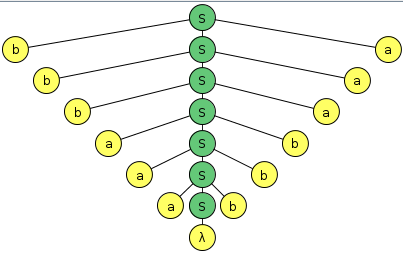
\includegraphics[width=0.8\textwidth]{img/eje_a_caso1.png}
        \end{minipage}
        } \\
         $ S \to bSa$ & bSa & \\
         $ S \to bSa$ & b bSa a & \\
         $ S \to bSa$ & bb bSa aa &\\
         $ S \to aSb$ & bbb aSb aaa &\\
         $ A \to aSb$ & bbba aSb baaa &\\
         $ A \to aSb$ & bbbaa aSb bbaaa &\\
         $ S \to \varepsilon$ & bbbaaabbbaaa &\\
         \hline
        \end{tabular}
        \\
        \begin{tabular}{|p{5cm}|p{5cm}|p{5cm}|  }
        \hline
        \multicolumn{3}{|c|}{Cadena con ubicación de $ba$'s  concatenada con $a$'s seguidas de $b$'s externamente : aabababb} \\
        \hline
        Producción & Derivación & Árbol\\
        \hline
        $ Inicio \to S$ & S & \multirow{7}{*}{
        \begin{minipage}{.3\textwidth}
        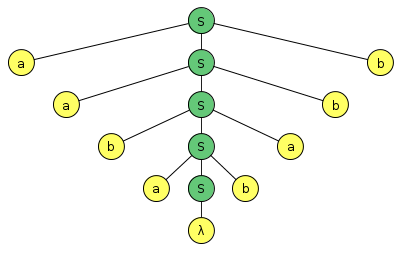
\includegraphics[width=0.8\textwidth]{img/eje_a_caso2.png}
        \end{minipage}
        } \\
         $ S \to aSb$ & aSb & \\
         $ S \to aSb$ & aaSbb S & \\
         $ S \to bSa$ & aabSabb&\\
         $ S \to aSb$ & aabaSbabb &\\
         $ S \to \varepsilon$ & aabababb &\\
         &&\\
         \hline
        \end{tabular}
        \\
        \begin{tabular}{|p{5cm}|p{5cm}|p{5cm}|  }
        \hline
        \multicolumn{3}{|c|}{Cadena con ubicación de $ab$'s  concatenada con $ba$'s en los extremos : baababba} \\
        \hline
        Producción & Derivación & Árbol\\
        \hline
        $ Inicio \to S$ & S & \multirow{7}{*}{
        \begin{minipage}{.3\textwidth}
        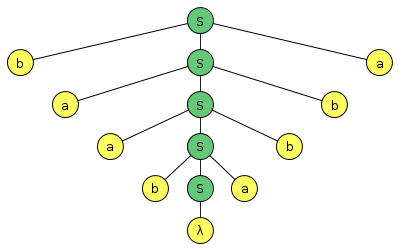
\includegraphics[width=0.8\textwidth]{img/eje_a_caso3.png}
        \end{minipage}
        } \\
         $ S \to bSa$ & bSa & \\
         $ S \to aSb$ & baSba S & \\
         $ S \to aSb$ & baaSbba&\\
         $ S \to bSa$ & baabSabba &\\
         $ S \to \varepsilon$ & baababba &\\
         &&\\
         \hline
        \end{tabular}
	    
	    \item $L = \{w |$ el tamaño de $w$ es impar y el símbolo del medio es $a \}$
	    
	    Gramática
	    \begin{itemize}
            \item $S \to \ ASA \ | \ a$
            \item $A \to \ a \ | \ b $
        \end{itemize}
        
        Derivación \\ 
        
        Para los casos mas pequeños por ejempo decir que la ocurrencia impar tambien puede ser tomado como el unico valor permitido $a$.
        
        \[ 
            S \Rightarrow_{lm} a
        \]
        
        Igualmente para el caso de tener solo $b$'s
        \[ 
            S \Rightarrow_{lm} ASA \Rightarrow_{lm} bSA \Rightarrow_{lm} baA \Rightarrow_{lm} bab
        \]
        Igualmente para el caso de tener solo $a$'s
        \[ 
            S \Rightarrow_{lm} ASA \Rightarrow_{lm} aSA \Rightarrow_{lm} aaA \Rightarrow_{lm} aaa
        \]
        
        O ambos
        \[ 
            S \Rightarrow_{lm} ASA \Rightarrow_{lm} aSA \Rightarrow_{lm} aaA \Rightarrow_{lm} aab
        \]
        
        Se presentan algunos casos mas extensos
        
        \begin{tabular}{|p{10cm}|p{5cm}| }
        \hline
         Cadena con cualquier cantidad de $a$'s y $b$'s: abbabba &  \\
         \hline
        
            \begin{tabular}{p{4cm}|p{5cm} }
             
             Producción & Derivación\\
             \hline
             
             $ Inicio \to S$ & S \\
             $ S \to ASA$ & ASA \\
             $ S \to ASA$ & AASAA \\
             $ S \to ASA$ & AAASAAA \\
             $ A \to a$ & aAASAAA \\
             $ A \to b$ & abASAAA \\
             $ A \to b$ & abbSAAA \\
             $ S \to a$ & abbaAAA \\
             $ A \to b$ & abbabAA \\
             $ A \to b$ & abbabbA \\
             $ A \to a$ & abbabbb  \\
             
            \end{tabular}
            &
            \begin{minipage}{.5\textwidth} \begin{figure}[H]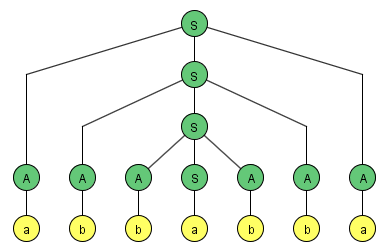
\includegraphics[scale=0.50]{img/2b1.PNG}\end{figure} \end{minipage}
            \\
            \hline
        \end{tabular}
        
        \begin{tabular}{|p{10cm}|p{5cm}| }
        \hline
        Cadena con $a$'s y $b$'s en cada lado: bbaaa &  \\
         \hline
            \begin{tabular}{p{4cm}|p{5cm}  }
             Producción & Derivación\\
             \hline
             $ Inicio \to S$ & S \\
             $ S \to ASA$ & ASA \\
             $ S \to ASA$ & AASAA \\
             $ A \to b$ & bASAA \\
             $ A \to b$ & bbSAA \\
             $ S \to a$ & bbaAA \\
             $ A \to a$ & bbaaA \\
             $ A \to a$ & bbaaa \\
             
            \end{tabular}
            &
            \begin{minipage}{.5\textwidth} \begin{figure}[H]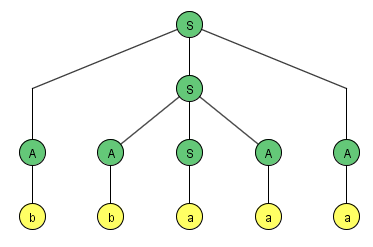
\includegraphics[scale=0.50]{img/2b2.PNG}\end{figure} \end{minipage}
            \\
            \hline
        \end{tabular}
        \\
        
        \begin{tabular}{|p{10cm}|p{5cm}| }
        \hline
            Cadena grande de $a$'s y $b$'s: aabbbabbaaa &  \\
         \hline
            \begin{tabular}{p{4cm}|p{5cm}  }
             Producción & Derivación\\
             \hline
             $ Inicio \to S$ & S \\
             $ S \to ASA$ & ASA \\
             $ S \to ASA$ & AASAA \\
             $ S \to ASA$ & AAASAAA \\
             $ S \to ASA$ & AAAASAAAA \\
             $ S \to ASA$ & AAAAASAAAAA \\
             $ A \to a$ & aAAAASAAAAA \\
             $ A \to a$ & aaAAASAAAAA \\
             $ A \to b$ & aabAASAAAAA \\
             $ A \to b$ & aabbASAAAAA \\
             $ A \to b$ & aabbbSAAAAA \\
             $ S \to a$ & aabbbaAAAAA \\
             $ A \to b$ & aabbbabAAAA \\
             $ A \to b$ & aabbbabbAAA \\
             $ A \to a$ & aabbbabbaAA \\
             $ A \to a$ & aabbbabbaaA \\
             $ A \to a$ & aabbbabbaa \\
             
            \end{tabular}
            &
            \begin{minipage}{.5\textwidth} \begin{figure}[H]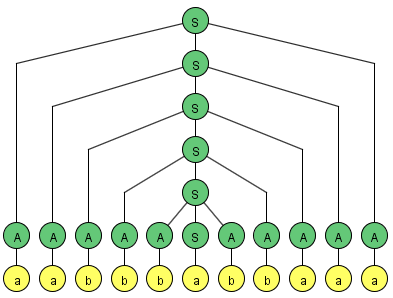
\includegraphics[scale=0.50]{img/2b3.PNG}\end{figure} \end{minipage}
            \\
            \hline
        \end{tabular}
        
	    
	    \item $L = \{w | w$ posee, máximo, 2 ocurrencias de $a\}$
	    
	   
	    Gramática
	    \begin{itemize}
            \item $S \to \ \epsilon \ | \ BXBXB$
            \item $B \to \ Bb \ | \ \epsilon$
            \item $X \to \ a \ | \ \epsilon$
        \end{itemize}
        Derivación \\ \\
        \begin{tabular}{|p{3.5cm}|p{3.5cm}|p{8cm}|  }
        
         \hline
         \multicolumn{3}{|c|}{Cadena con dos  $a$'s: babba} \\
         \hline
         Producción & Derivación & Árbol\\
         \hline
         
         \begin{itemize}[label={}]
             \item $ S \to BXBXB$ 
             \item $ B \to Bb$ 
             \item $ B \to Bb$ 
             \item $ B \to Bb$ 
             \item $ B \to \epsilon $ 
             \item $ X \to a$	
             \item $ B \to \epsilon$ 
             \item $ X \to a$	
             \item $ B \to \epsilon$ 
        \end{itemize}
        &
        \begin{itemize}[label={}]
             \item BXBXB 
             \item BXBbXB 
             \item BbXBbXB 
             \item BbXBbbXB 
             \item bXBbbXB 
             \item baBbbXB 
             \item babbXB 
             \item babbaB 
             \item babba 
        \end{itemize}
        
        &
        \begin{itemize}[label={}]
             \item 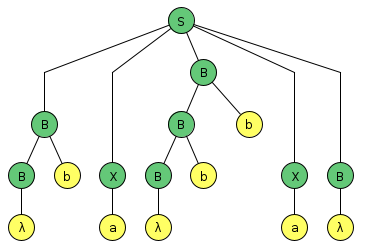
\includegraphics[scale=0.40]{img/2c-babba.png}
        \end{itemize}
      \\ \hline
        \end{tabular}
        \\ \\
        
        \begin{tabular}{|p{3.5cm}|p{3.5cm}|p{8cm}|  }
         \hline
         \multicolumn{3}{|c|}{Cadena con una  $a$: bbbbab} \\
         \hline
         Producción & Derivación & Árbol\\
         \hline
         \begin{itemize}[label={}]
             
         \item $S\to BXBXB$ 
         \item $B \to Bb$	
         \item $B \to Bb$	
         \item $B \to Bb$	
         \item $B \to Bb$	
         \item $B \to Bb$	
         \item $B \to \epsilon$	
         \item $X \to \epsilon$	
         \item $B \to \epsilon$	
         \item $X \to a$	
         \item $B \to \epsilon$
         
        \end{itemize}
        &
         \begin{itemize}[label={}]
             
             \item	BXBXB 
             \item BbXBXB 
             \item BbXBbXB 
             \item BbbXBbXB 
             \item BbbXBbbXB 
             \item BbbXBbbXBb 
             \item bbXBbbXBb 
             \item bbBbbXBb 
             \item bbbbXBb 
             \item bbbbaBb 
             \item bbbbab 
        \end{itemize}
        &
         \begin{itemize}[label={}]
             \item 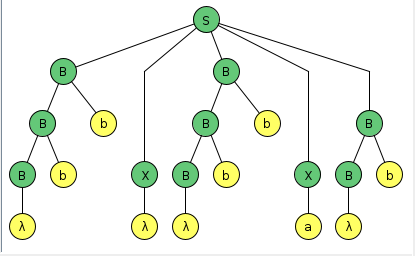
\includegraphics[scale=0.40]{img/2c-bbbbab.png}
        \end{itemize}
        \\ \hline
        \end{tabular}
        \\
        \begin{tabular}{|p{3.5cm}|p{3.5cm}|p{8cm}|  }
         \hline
         \multicolumn{3}{|c|}{Cadena sin ninguna  $a$'s: bbb} \\
         \hline
         Producción & Derivación & Árbol\\
         \hline
          \begin{itemize}[label={}]
             
              \item $ S \to BXBXB$ 
         \item $ B \to Bb$ 
         \item $ B \to Bb$ 
         \item $ B \to Bb$ 
         \item $ B \to \epsilon $ 
         \item $ X \to \epsilon$	
         \item $ B \to \epsilon$ 
         \item $ X \to \epsilon$
         \item $ B \to \epsilon$
         
        \end{itemize}
        &
         \begin{itemize}[label={}]
              \item BXBXB
         \item	BbXBXB 
         \item	BbXBbXB 
         \item	BbXBbXBb 
         \item bXBbXBb 
         \item bBbXBb 
         \item bbXBb 
         \item bbBb 
         \item bbb 
         
        \end{itemize}
        &
         \begin{itemize}[label={}]
             \item 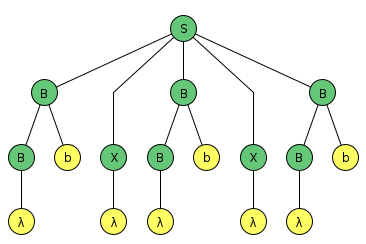
\includegraphics[scale=0.40]{img/2c-bbb.png}
        \end{itemize}
        \\ \hline
        \end{tabular}
        
	    \item $L = \{a^nb^mc^md^n|$ $n \geq 0$ e $m > 0\}$
	    
	    Gramática
    	    \begin{itemize}
        	    \item $G \rightarrow MbIcN$
        	    \item $I \rightarrow bIc | \varepsilon$
        	    \item $M \rightarrow aM | \varepsilon$
        	    \item $N \rightarrow dN | \varepsilon$
    	    \end{itemize}
            
            Derivación \\ \\
            
            Para el caso en que sol puede ser $b$ y $c$'s siendo $a$'s y $d$'s ceros
            
            \[ 
                I \Rightarrow_{lm} bIc | \varepsilon 
            \]
            
            Para el caso en donde puede haber almenos $b$ y $c$'s y varios casos de $a$ y $d$'s respetando la posicion
            \[ 
                G \Rightarrow_{lm} MIN 
            \]
            Y para el caso en donde se requiere varias veces las $a$ y $d$'s
            \[ 
                M \Rightarrow_{lm} aM | \varepsilon
                N \Rightarrow_{lm} dN | \varepsilon
            \]
            
            Se presentan algunos casos mas extensos
            
            \begin{tabular}{|p{5cm}|p{5cm}|p{5cm}|  }
            \hline
            \multicolumn{3}{|c|}{Cadena con solo las letras $b$ y $c$ sin contar con $a$ y $d$ bbbccc} \\
            \hline
            Producción & Derivación & Árbol\\
            \hline
            $ Inicio \to G$ & G & \multirow{5}{*}{
            \centering
            \begin{minipage}{.3\textwidth}
            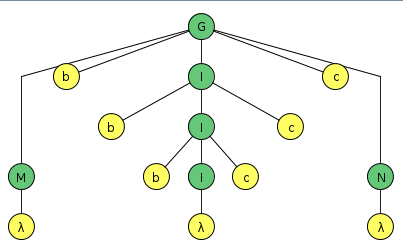
\includegraphics[width=0.8\textwidth]{img/eje_d_caso1.png}
            \end{minipage}
            } \\
             $ G \to MbIcN$ & MbIcN & \\
             $ I \to bIc$ & MbbIccN & \\
             $ I \to bIc$ & MbbbIcccN & \\
             $ M \to \varepsilon$ & bbbIcccN &\\
             $ I \to \varepsilon$ & bbbcccN &\\
             $ N \to \varepsilon$ & bbbccc &\\
             \hline
            \end{tabular}
            \\
            \begin{tabular}{|p{5cm}|p{5cm}|p{5cm}|  }
            \hline
            \multicolumn{3}{|c|}{Cadena con ubicación de $b$'s  y $c$'s seguidas concatenado con $a$'s y $d$ al extremo : abbbcccd} \\
            \hline
            Producción & Derivación & Árbol\\
            \hline
            $ Inicio \to G$ & G & \multirow{9}{*}{
            \begin{minipage}{.3\textwidth}
            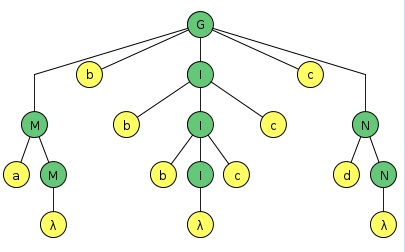
\includegraphics[width=0.8\textwidth]{img/eje_d_caso2.png}
            \end{minipage}
            } \\
             $ G \to MbIcN$ & MbIcN & \\
             $ I \to bIc$ & MbcIccN S & \\
             $ M \to aM$ & aMbcIccN&\\
             $ I \to bIc$ & aMbbbIcccN&\\
             $ N \to dN$ & aMbbbIcccdN&\\
             $ M \to \varepsilon$ & abbbIcccdN&\\
             $ I \to \varepsilon$ & abbbcccdN&\\
             $ N \to \varepsilon$ & abbbcccd&\\
             &&\\
             \hline
            \end{tabular}
            \\
            \begin{tabular}{|p{5cm}|p{5cm}|p{5cm}|  }
            \hline
            \multicolumn{3}{|c|}{Cadena con ubicación unica $b$'  y $c$' concatenado con $a$'s y $d$'c al extremo: aaabcddd} \\
            \hline
            Producción & Derivación & Árbol\\
            \hline
            $ Inicio \to G$ & G & \multirow{10}{*}{
            \begin{minipage}{.3\textwidth}
            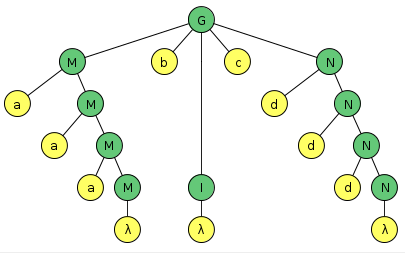
\includegraphics[width=0.8\textwidth]{img/eje_d_caso3.png}
            \end{minipage}
            } \\
             $ G \to MbIcN$ & MbIcN & \\
             $ M \to aM$ & aMbIcN S & \\
             $ N \to dN$ & aMbIcdN&\\
             $ M \to aM$ & aaMbIcdN &\\
             $ N \to dN$ & aaMbIcddN &\\
             $ M \to aM$ & aaaMbIcddN &\\
             $ N \to dN$ & aaaMbIcdddN &\\
             $ M \to \varepsilon$ & aaabIcdddN &\\
             $ I \to \varepsilon$ & aaabcdddN &\\
             $ N \to \varepsilon$ & aaabcddd &\\
             &&\\
             \hline
            \end{tabular}
	    
	    \item $L = \{a^nb^m | 0 \leq n \leq m \leq 2n\}$
	    Gramática
	    \begin{itemize}
            \item $S \to \ \epsilon \ | \ aSR$
            \item $R \to \ bb \ | \ b$
            
        \end{itemize}
        Derivación
        \\ \\ 
        \begin{tabular}{|p{3.5cm}|p{3.5cm}|p{8cm}|  }
         \hline
         \multicolumn{3}{|c|}{Cadena con m = n : ab} \\
         \hline
         Producción & Derivación & Árbol\\
         \hline
         \begin{itemize}[label={}]
             
             \item $ S \to aSR$ 
         \item $ S \to \epsilon$
         \item $ R \to b$	
         
         
        \end{itemize}
        &
        \begin{itemize}[label={}]
             
             \item	aSR 
         \item aR 
         \item ab 
         
        \end{itemize}
        &
         \begin{itemize}[label={}]
             \item 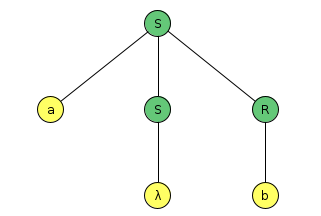
\includegraphics[scale=0.40]{img/2e-ab.png}
        \end{itemize}
        \\ \hline
        \end{tabular}
        \\ \\
        \begin{tabular}{|p{3.5cm}|p{3.5cm}|p{8cm}|  }
         \hline
         \multicolumn{3}{|c|}{Cadena con m $>$ n : aabbb} \\
         \hline
         Producción & Derivación & Árbol\\
         \hline
         \begin{itemize}[label={}]
             
             \item $ S \to aSR$ 
         \item $ S \to aSR$ 
         \item $ S \to \epsilon$
         \item $ R \to bb$	
         \item $ R \to b$	
         
         
        \end{itemize}
        &
        \begin{itemize}[label={}]
             
             \item	aSR 
         \item	aaSRR 
         \item aaRR 
         \item aabbR 
         \item aabbb 
         
         
        \end{itemize}
        &
         \begin{itemize}[label={}]
             \item 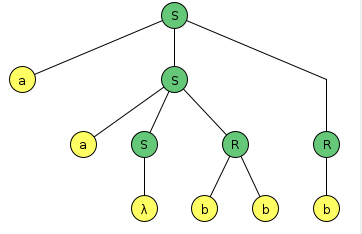
\includegraphics[scale=0.40]{img/2e-aabbb.png}
        \end{itemize}
        
         
         \\ \hline
        \end{tabular}
        \\ \\
        \begin{tabular}{|p{3.5cm}|p{3.5cm}|p{8cm}|  }
         \hline
         \multicolumn{3}{|c|}{Cadena con m = 2n : aabbbb} \\
         \hline
         Producción & Derivación & Árbol\\
         \hline
         
         \begin{itemize}[label={}]
             
             \item $ S \to aSR$ 
         \item $ S \to aSR$ 
         \item $ S \to \epsilon$ 
         \item $ R \to bb$	
         \item $ R \to bb$	
         
         
        \end{itemize}
        &
        \begin{itemize}[label={}]
             \item	aSR 
         \item aaSRR 
         \item	aaRR 
         \item aabbR 
         \item aabbbb 
         
        \end{itemize}
        &
         \begin{itemize}[label={}]
             \item 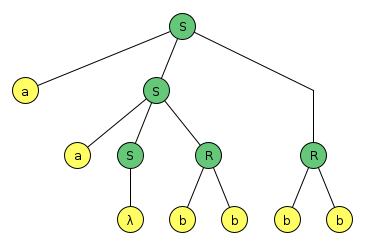
\includegraphics[scale=0.40]{img/2e-aabbbb.png}
        \end{itemize}
        
         
        \\ \hline
        \end{tabular}
	    \item $L = \{a^ib^jc^k| k = i + j\}$
	    
	    Gramática
    	    \begin{itemize}
        	    \item $S \rightarrow aSc $
        	    \item $S \rightarrow B | \varepsilon$
        	    \item $B \rightarrow bBc | \varepsilon$
        	    
    	    \end{itemize}
            
            Derivación \\ \\
            
            Para el caso del conteo de las $a$'s y como primera posición de la cadena antes de las $c$'s
            
            \[ 
                S \Rightarrow_{lm} aSc
            \]
            
            Para el caso del conteo de las $b$'s con recursividad llamamos a $B$ y como segunda posición de la cadena antes de las $c$'s
            \[ 
                B \Rightarrow_{lm} bBc | \varepsilon 
            \]
            
            Se presentan algunos casos mas extensos
            
            \begin{tabular}{|p{5cm}|p{5cm}|p{5cm}|  }
            \hline
            \multicolumn{3}{|c|}{Cadena con tres $a$'s y dos $b$'s resulta cinco $c$'s aaabbccccc} \\
            \hline
            Producción & Derivación & Árbol\\
            \hline
            $ Inicio \to S$ & S & \multirow{7}{*}{
            \centering
            \begin{minipage}{.3\textwidth}
            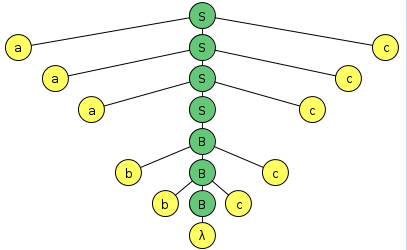
\includegraphics[width=0.8\textwidth]{img/eje_f_caso1.png}
            \end{minipage}
            } \\
             $ S \to aSc$ & aSc & \\
             $ S \to aSc$ & aaScc & \\
             $ S \to aSc$ & aaaSccc & \\
             $ S \to B$ & aaaBccc & \\
             $ B \to bBc$ & aaabBcccc & \\
             $ B \to bBc$ & aaabbBccccc & \\
             $ B \to \varepsilon$ & aaabbccccc & \\
             \hline
            \end{tabular}
            \\
            \begin{tabular}{|p{5cm}|p{5cm}|p{5cm}|  }
            \hline
            \multicolumn{3}{|c|}{Cadena con una unica letra $b$ eso resulta en una unica $c$: bc} \\
            \hline
            Producción & Derivación & Árbol\\
            \hline
            $ Inicio \to S$ & S & \multirow{3}{*}{
            \begin{minipage}{.3\textwidth}
            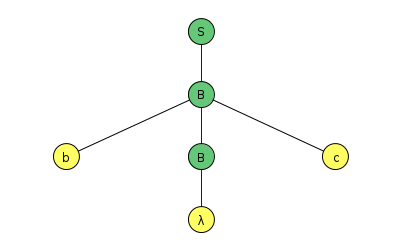
\includegraphics[width=0.8\textwidth]{img/eje_f_caso2.png}
            \end{minipage}
            } \\
             $ S \to B$ &  EGc& \\
             $ B \to bBc$ & bGc S & \\
             $ B \to \varepsilon$ & bc&\\
             &&\\
             \hline
            \end{tabular}
            \\
            \begin{tabular}{|p{5cm}|p{5cm}|p{5cm}|  }
            \hline
            \multicolumn{3}{|c|}{Cadena con solo 5 $a$'s  y unica $b$ concatenado con 5 $c$'s extremo: aaaaabcccccc} \\
            \hline
            Producción & Derivación & Árbol\\
            \hline
            $ Inicio \to S$ & S & \multirow{11}{*}{
            \begin{minipage}{.3\textwidth}
            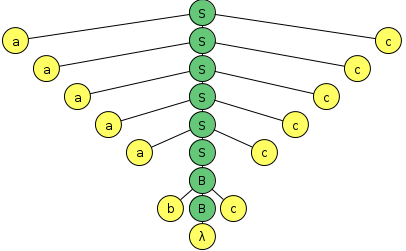
\includegraphics[width=0.8\textwidth]{img/eje_f_caso3.png}
            \end{minipage}
            } \\
             $ S \to aSc$ & aSc & \\
             $ S \to aSc$ & aaScc & \\
             $ S \to aSc$ & aaaSccc & \\
             $ S \to aSc$ & aaaaScccc & \\
             $ S \to aSc$ & aaaaaSccccc & \\
             
             $ S \to B$ & aaaaaBccccc & \\
             $ B \to bBc$ & aaaaabBcccccc & \\
             $ b \to \varepsilon$ & aaaaabcccccc & \\
             \hline
            \end{tabular}
	    
	    \item $L = \{a^nb^{n+m}c^m | n, m \geq 0\}$
	    Gramática
	    \begin{itemize}
            \item $S \to \ \epsilon \ | \ XY$
            \item $X \to \ aXb \ | \ \epsilon $
            \item $Y \to \ bYc \ | \ \epsilon $
        \end{itemize}
        Derivación
        \\ \\ 
        \begin{tabular}{|p{3.5cm}|p{3.5cm}|p{8cm}|  }
         \hline
         \multicolumn{3}{|c|}{Cadena con n = 0, m = 3 : bbbccc} \\
         \hline
         Producción & Derivación & Árbol\\
         \hline
         \begin{itemize}[label={}]
             
             
         \item $ S \to XY$
         \item $ Y \to bYc$	
         \item $ Y \to bYc$	
         \item $ Y \to bYc$	
         \item $ X \to \epsilon$	
         \item $ Y \to \epsilon$	
         
         
        \end{itemize}
        &
        \begin{itemize}[label={}]
             
             
         \item	XY 
         \item	XbYc 
         \item	XbbYcc 
         \item	XbbbYccc 
         \item	bbbYccc 
         \item	bbbccc 
         
         
        \end{itemize}
        &
         \begin{itemize}[label={}]
             \item 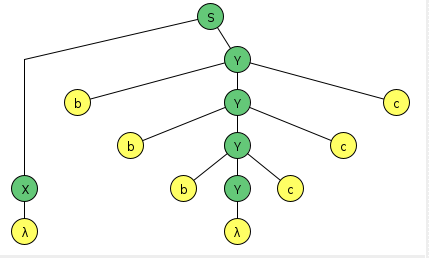
\includegraphics[scale=0.40]{img/2g-bbbccc.png}
        \end{itemize}
        
        \\ \hline
        \end{tabular}
        \\ \\
        \begin{tabular}{|p{3.5cm}|p{3.5cm}|p{8cm}|  }
         \hline
         \multicolumn{3}{|c|}{Cadena con m = 0, n = 2 : aabb} \\
         \hline
         Producción & Derivación & Árbol\\
         \hline
         \begin{itemize}[label={}]
             
             
         \item $ S \to XY$	
         \item $ X \to aXb$	
         \item $ X \to aXb$	
         \item $ X \to \epsilon$
         \item $ Y \to \epsilon$
         
         
        \end{itemize}
        &
        \begin{itemize}[label={}]
             
             
         \item	XY 
         \item	aXbY 
         \item	aaXbbY 
         \item	aabbY 
         \item	aabb 
         
         
        \end{itemize}
        &
         \begin{itemize}[label={}]
             \item 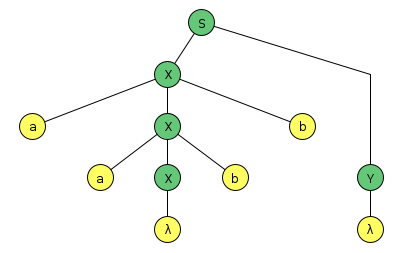
\includegraphics[scale=0.40]{img/2g-aabb.png}
        \end{itemize}
        
         
         \\ \hline
        \end{tabular}
        \\ \\
        \begin{tabular}{|p{3.5cm}|p{3.5cm}|p{8cm}|  }
         \hline
         \multicolumn{3}{|c|}{Cadena con m = 1, n = 3 : aaabbbbc} \\
         \hline
         Producción & Derivación & Árbol\\
         \hline
         \begin{itemize}[label={}]
             
             \item $ S \to XY$	
         \item $ X \to aXb$ 
         \item $ X \to aXb$ 
         \item $ X \to aXb$ 
         \item $ Y \to bYc$ 
         \item $ X \to \epsilon$ 
         \item $ Y \to \epsilon$ 
         
        \end{itemize}
        &
        \begin{itemize}[label={}]
             
             \item XY 
         	\item aXbY 
         \item	aaXbbY 
         \item	aaaXbbbY 
         \item	aaaXbbbbYc 
         \item	aaabbbbYc 
         \item	aaabbbbc 
         
        \end{itemize}
        &
         \begin{itemize}[label={}]
             \item 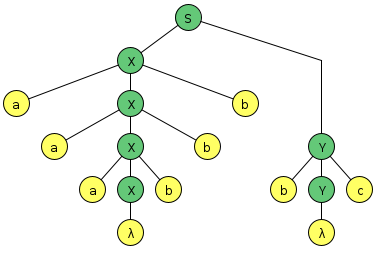
\includegraphics[scale=0.40]{img/2g-aaabbbbc.png}
        \end{itemize}
        
         
        \\ \hline
        \end{tabular}
	\end{enumerate}
    
    
% \begin{table}[]
%     \begin{tabular}{lllllllllll}
%     (a) & $ L_1 : \{a^ib | i \geq 1\}$ \dotfill & $\boxtimes$ 1 & \mbox{\ooalign{$\checkmark$\cr\hidewidth$\square$\hidewidth\cr}} 2 & {$\square$}\raisebox{.15ex}{\hspace{0.1em}$\checkmark$} 3 & {$\square$}\raisebox{.15ex}{\hspace{0.1em}$\checkmark$} 4 & {$\square$}\raisebox{.15ex}{\hspace{0.1em}$\checkmark$} 5 & {$\square$}\raisebox{.15ex}{\hspace{0.1em}$\checkmark$} 6 & {$\square$}\raisebox{.15ex}{\hspace{0.1em}$\checkmark$} 7 & {$\square$}\raisebox{.15ex}{\hspace{0.1em}$\checkmark$} 8 & {$\square$}\raisebox{.15ex}{\hspace{0.1em}$\checkmark$} 9 \\
%     (b) & $ L_2 : \{(ab)^ia | i \geq 0\}$ \dotfill & {$\square$}\raisebox{.15ex}{\hspace{0.1em}$\checkmark$} 1 & {$\square$}\raisebox{.15ex}{\hspace{0.1em}$\checkmark$} 2 & {$\square$}\raisebox{.15ex}{\hspace{0.1em}$\checkmark$} 3 & {$\square$}\raisebox{.15ex}{\hspace{0.1em}$\checkmark$} 4 & {$\square$}\raisebox{.15ex}{\hspace{0.1em}$\checkmark$} 5 & {$\square$}\raisebox{.15ex}{\hspace{0.1em}$\checkmark$} 6 & {$\square$}\raisebox{.15ex}{\hspace{0.1em}$\checkmark$} 7 & {$\square$}\raisebox{.15ex}{\hspace{0.1em}$\checkmark$} 8 & {$\square$}\raisebox{.15ex}{\hspace{0.1em}$\checkmark$} 9 \\
%     (c) & $ L_3 : \{a^ib | i \geq 2\}$ \dotfill & {$\square$}\raisebox{.15ex}{\hspace{0.1em}$\checkmark$} 1 & {$\square$}\raisebox{.15ex}{\hspace{0.1em}$\checkmark$} 2 & {$\square$}\raisebox{.15ex}{\hspace{0.1em}$\checkmark$} 3 & {$\square$}\raisebox{.15ex}{\hspace{0.1em}$\checkmark$} 4 & {$\square$}\raisebox{.15ex}{\hspace{0.1em}$\checkmark$} 5 & {$\square$}\raisebox{.15ex}{\hspace{0.1em}$\checkmark$} 6 & {$\square$}\raisebox{.15ex}{\hspace{0.1em}$\checkmark$} 7 & {$\square$}\raisebox{.15ex}{\hspace{0.1em}$\checkmark$} 8 & {$\square$}\raisebox{.15ex}{\hspace{0.1em}$\checkmark$} 9 \\
%     (d) & $ L_4 : \{a^iba^j| i \geq 1, j \geq 0\}$ \dotfill & {$\square$}\raisebox{.15ex}{\hspace{0.1em}$\checkmark$} 1 & {$\square$}\raisebox{.15ex}{\hspace{0.1em}$\checkmark$} 2 & {$\square$}\raisebox{.15ex}{\hspace{0.1em}$\checkmark$} 3 & {$\square$}\raisebox{.15ex}{\hspace{0.1em}$\checkmark$} 4 & {$\square$}\raisebox{.15ex}{\hspace{0.1em}$\checkmark$} 5 & {$\square$}\raisebox{.15ex}{\hspace{0.1em}$\checkmark$} 6 & {$\square$}\raisebox{.15ex}{\hspace{0.1em}$\checkmark$} 7 & {$\square$}\raisebox{.15ex}{\hspace{0.1em}$\checkmark$} 8 & {$\square$}\raisebox{.15ex}{\hspace{0.1em}$\checkmark$} 9 \\
%     (e) & $ L_5 : \{a^ib | i \geq 0\}$ \dotfill & {$\square$}\raisebox{.15ex}{\hspace{0.1em}$\checkmark$} 1 & {$\square$}\raisebox{.15ex}{\hspace{0.1em}$\checkmark$} 2 & {$\square$}\raisebox{.15ex}{\hspace{0.1em}$\checkmark$} 3 & {$\square$}\raisebox{.15ex}{\hspace{0.1em}$\checkmark$} 4 & {$\square$}\raisebox{.15ex}{\hspace{0.1em}$\checkmark$} 5 & {$\square$}\raisebox{.15ex}{\hspace{0.1em}$\checkmark$} 6 & {$\square$}\raisebox{.15ex}{\hspace{0.1em}$\checkmark$} 7 & {$\square$}\raisebox{.15ex}{\hspace{0.1em}$\checkmark$} 8 & {$\square$}\raisebox{.15ex}{\hspace{0.1em}$\checkmark$} 9 \\
%     (f) & $ L_6 : \{a^ib^j| i \geq 0, j > 0\}$ \dotfill & {$\square$}\raisebox{.15ex}{\hspace{0.1em}$\checkmark$} 1 & {$\square$}\raisebox{.15ex}{\hspace{0.1em}$\checkmark$} 2 & {$\square$}\raisebox{.15ex}{\hspace{0.1em}$\checkmark$} 3 & {$\square$}\raisebox{.15ex}{\hspace{0.1em}$\checkmark$} 4 & {$\square$}\raisebox{.15ex}{\hspace{0.1em}$\checkmark$} 5 & {$\square$}\raisebox{.15ex}{\hspace{0.1em}$\checkmark$} 6 & {$\square$}\raisebox{.15ex}{\hspace{0.1em}$\checkmark$} 7 & {$\square$}\raisebox{.15ex}{\hspace{0.1em}$\checkmark$} 8 & {$\square$}\raisebox{.15ex}{\hspace{0.1em}$\checkmark$} 9 \\
%     (g) & $ L_7 : \{(ab)^i| i \geq 0\}$ \dotfill {$\square$}\raisebox{.15ex}{\hspace{0.1em}$\checkmark$} 1 & {$\square$}\raisebox{.15ex}{\hspace{0.1em}$\checkmark$} 2 & {$\square$}\raisebox{.15ex}{\hspace{0.1em}$\checkmark$} 3 & {$\square$}\raisebox{.15ex}{\hspace{0.1em}$\checkmark$} 4 & {$\square$}\raisebox{.15ex}{\hspace{0.1em}$\checkmark$} 5 & {$\square$}\raisebox{.15ex}{\hspace{0.1em}$\checkmark$} 6 & {$\square$}\raisebox{.15ex}{\hspace{0.1em}$\checkmark$} 7 & {$\square$}\raisebox{.15ex}{\hspace{0.1em}$\checkmark$} 8 & {$\square$}\raisebox{.15ex}{\hspace{0.1em}$\checkmark$} 9 \\
%     \end{tabular}
%     \end{table}
	
	%\clearpage
	%\bibliographystyle{apalike}
	\bibliographystyle{IEEEtranN}
	\bibliography{biblio}
		
	
\end{document}